\documentclass[11pt,a4paper]{article}

\usepackage[utf8]{inputenc}
\usepackage[T1]{fontenc}
\usepackage[french]{babel}
\usepackage{amsmath,amssymb}
\usepackage{graphicx}
\usepackage[a4paper,margin=2.5cm]{geometry}
\usepackage{hyperref}
\hypersetup{colorlinks=true,linkcolor=black,urlcolor=blue,citecolor=black}

% Mise en page un peu plus aeree : interligne et espacement entre paragraphes.
\linespread{1.05}
\setlength{\parskip}{0.6em}

\graphicspath{{figures_local/}}

\title{Projet Méthodes Stochastiques\\[0.3em]
       \large Deuxième modèle : le terme $\sigma\,dX_t$}
\author{Philippe \textsc{Lin} \and Sayna \textsc{Ren} \and Xuhong \textsc{Liu}}
\date{}

\begin{document}

\maketitle

\textit{Tous les résultats sont reproductibles dans le notebook de la partie 2 qui accompagne cette note, où l'on trouve l'ensemble des codes et des figures.}

\section*{Deuxième modèle (\texttt{virus6.csv})}

L'effet du virus est ici un peu plus complexe, le virus agissant aussi directement sur les victimes par un terme $\sigma\,dX_t$. Le système devient

\begin{equation}\label{eq:modele2}
  dV_t = V_t\left(\tfrac{2}{3} - \tfrac{4}{3}P_t + X_t\right)dt + \sigma\,dX_t,
  \qquad
  dP_t = P_t\left(-1 + V_t\right)dt.
\end{equation}

L'équation des prédateurs reste sans bruit, si bien que le pas de temps se récupère exactement comme dans le premier modèle, en moyennant $\Delta P_i/[P_i(-1+V_i)]$ là où le dénominateur n'est pas trop petit. On trouve $dt \approx 0{,}0154$ et $\tau \approx 30{,}8$. Cette fois les prédateurs s'éteignent, leur densité passant sous $0{,}01$ vers $t \approx 28$ (figure~\ref{fig:p2donnees}).

\begin{figure}[ht]
  \centering
  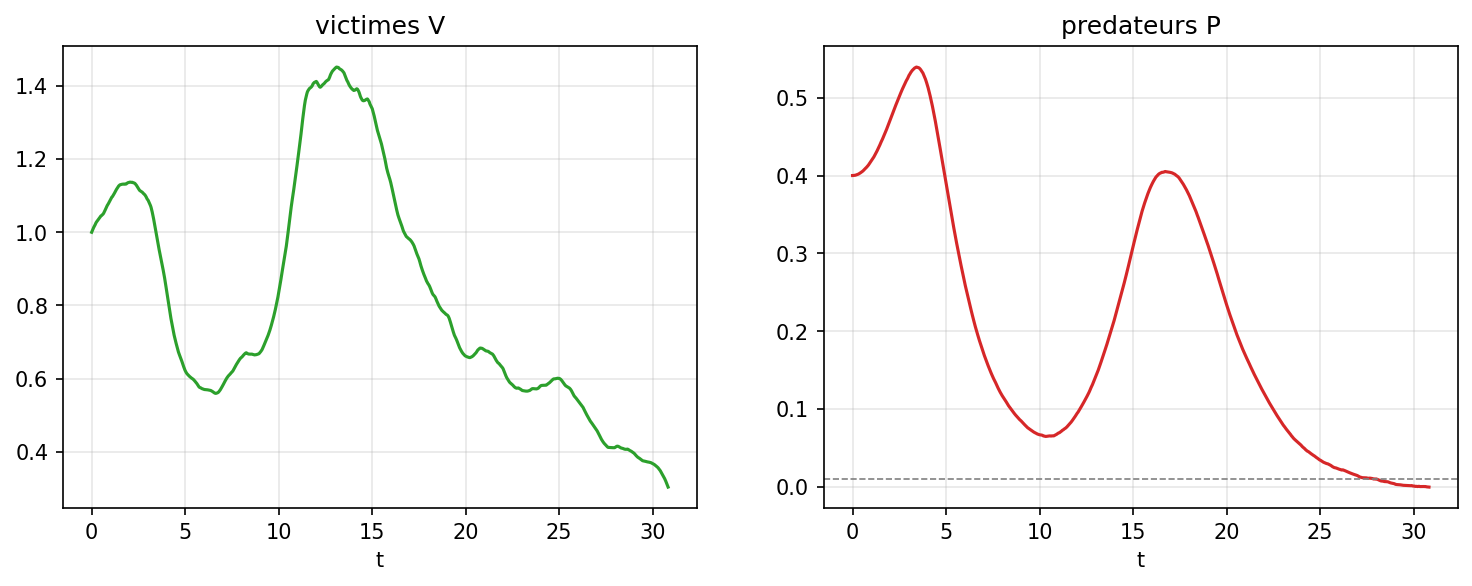
\includegraphics[width=\textwidth]{p2_donnees.png}
  \caption{Densités observées de victimes (gauche) et de prédateurs (droite) dans \texttt{virus6.csv}. Les prédateurs passent sous le seuil d'extinction $0{,}01$ (tirets) en fin d'intervalle.}
  \label{fig:p2donnees}
\end{figure}

\subsection*{Question 1 — évaluation de $\sigma$}

Dans \eqref{eq:modele2}, le seul terme portant une différentielle stochastique est $\sigma\,dX_t$, c'est donc le seul à contribuer à la variation quadratique de $V$,

\begin{equation}\label{eq:qv}
  [V]_\tau = \sigma^2\,[X]_\tau.
\end{equation}

La somme brute $\sum(\Delta V_i)^2$ est cependant dominée par la dérive lisse $V_t(\dots)dt$, qui n'a pas de variation quadratique mais en simule une à pas fini. Pour isoler la partie martingale, nous regardons les différences secondes $\Delta^2 V_i$, qui annulent une tendance lisse (d'ordre $dt^2$) mais gardent la partie brownienne (d'ordre $\sqrt{dt}$). En retranchant le cas sans bruit \texttt{virus4.csv} (où $\sigma = 0$) comme référence, l'excès de rugosité donne

\begin{equation}\label{eq:sigs}
  \sigma\,s \approx \sqrt{\frac{\sum (\Delta^2 V^{(6)}_i)^2 - \sum (\Delta^2 V^{(4)}_i)^2}{2\,\tau}} \approx 10^{-3},
\end{equation}

où $s$ désigne la diffusion du virus, c'est-à-dire l'intensité de sa partie brownienne. Cette variation quadratique ne fournit que le produit $\sigma\,s$. Le virus étant le même qu'au premier modèle, nous reprenons sa diffusion $s \approx 0{,}05$ estimée en partie 1, ce qui donne

\begin{center}
  $\sigma \approx 0{,}02.$
\end{center}

\textbf{À priori, $\sigma$ est petit}, l'apport direct du virus sur $V$ restant une perturbation modeste devant sa dérive.

\subsection*{Question 2 — une EDS pour le virus}

$\sigma$ étant petit, la reconstruction du premier modèle reste valable au premier ordre, le virus apparent $X_i \approx \Delta V_i/(V_i\,dt) - \tfrac{2}{3} + \tfrac{4}{3}P_i$ (figure~\ref{fig:p2virus}). Le virus part de $0$ et dérive régulièrement vers $\approx -1$, sans jamais revenir vers un niveau fixe. C'est cette intensité négative qui s'installe durablement qui finit par éteindre les prédateurs.

\begin{figure}[ht]
  \centering
  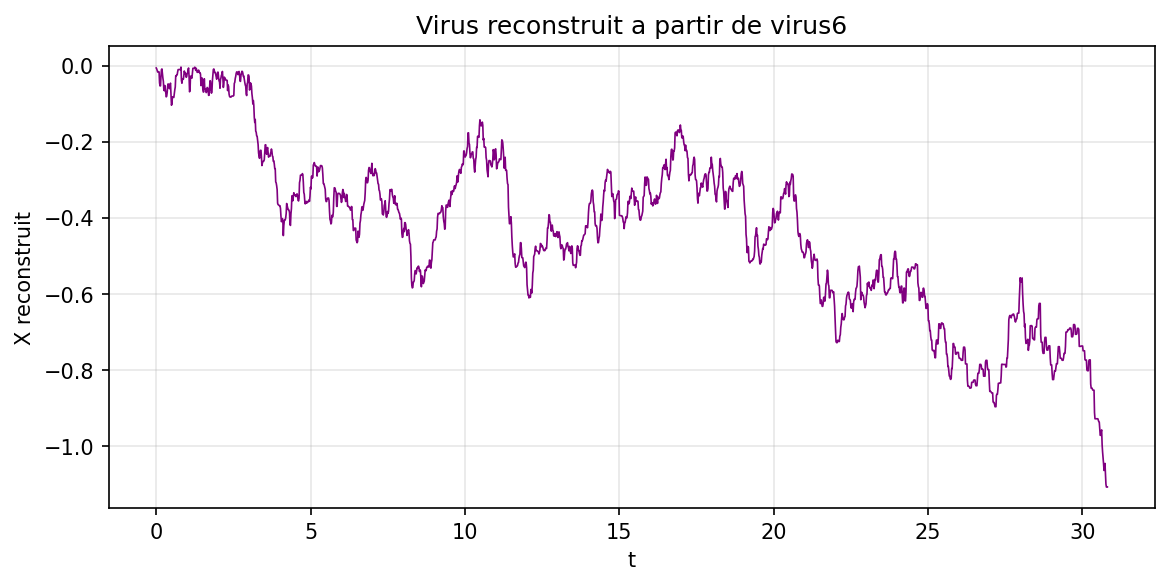
\includegraphics[width=0.8\textwidth]{p2_virus.png}
  \caption{Virus reconstruit à partir de \texttt{virus6.csv}. La trajectoire erre vers le bas sans retour à un niveau, à la manière d'une marche aléatoire avec dérive.}
  \label{fig:p2virus}
\end{figure}

L'absence de retour à la moyenne écarte un Ornstein-Uhlenbeck et oriente vers le modèle minimal d'un brownien avec dérive,

\begin{equation}\label{eq:eds2}
  dX_t = \nu\,dt + s\,dB_t.
\end{equation}

La dérive s'estime par la moyenne des différences, $\nu = \overline{\Delta X}/dt \approx -0{,}036$, et la dérive cumulée $\nu\tau \approx -1{,}1$ rend bien compte du niveau atteint en fin d'intervalle. Comme en partie 1, le test des résidus $\varepsilon_i = (\Delta X_i - \nu\,dt)/(s\sqrt{dt})$ contre $\mathcal N(0,1)$ donne une p-value de l'ordre de $10^{-24}$ et une corrélation entre résidus consécutifs de l'ordre de $0{,}26$ (figure~\ref{fig:p2residus}), donc le bruit n'est pas exactement gaussien ni indépendant.

\begin{figure}[ht]
  \centering
  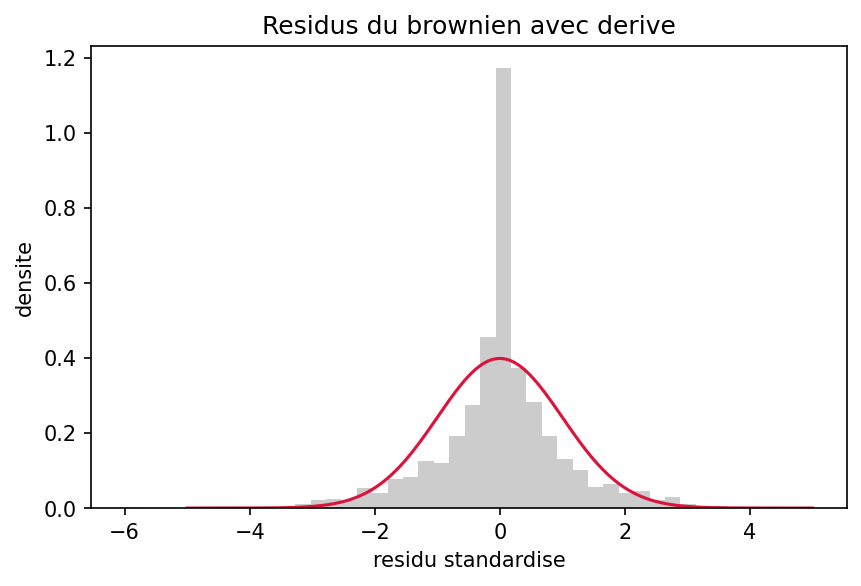
\includegraphics[width=0.55\textwidth]{p2_residus.png}
  \caption{Histogramme des résidus standardisés du brownien avec dérive, comparé à $\mathcal N(0,1)$.}
  \label{fig:p2residus}
\end{figure}

\textbf{À priori, on retient le brownien avec dérive comme modèle le plus simple,} avec la même réserve qu'en partie 1 sur la structure fine du bruit.

\subsection*{Question 3 — loi de $X_\tau$}

Sous le modèle~\eqref{eq:eds2}, l'intégration est immédiate, $X_\tau = X_0 + \nu\tau + s\,B_\tau$. L'intégrand devant le brownien étant déterministe, $X_\tau$ est une combinaison affine d'une gaussienne $B_\tau \sim \mathcal N(0,\tau)$, donc elle-même gaussienne,

\begin{equation}\label{eq:loi}
  X_\tau \sim \mathcal N\!\left(X_0 + \nu\tau,\ s^2\tau\right).
\end{equation}

Avec $X_0 = 0$, $\nu \approx -0{,}036$ et $s \approx 0{,}05$, on obtient une moyenne $\nu\tau \approx -1{,}1$ et un écart-type $s\sqrt{\tau} \approx 0{,}28$, soit

\begin{center}
  $X_\tau \sim \mathcal N(-1{,}1,\ 0{,}28^2).$
\end{center}

\textbf{À priori, on propose une loi normale pour $X_\tau$.} Une seule trajectoire ne permet pas de la valider, mais sa moyenne $\nu\tau$ coïncide avec la valeur reconstruite $X_\tau \approx -1{,}1$, et le caractère gaussien découle directement de la linéarité de l'EDS.

\subsection*{Bilan}

Le terme direct du virus est faible ($\sigma \approx 0{,}02$). Le virus lui-même se décrit au plus simple par un brownien avec dérive nettement négative, qui pousse l'intensité vers $\approx -1$ et précipite l'extinction des prédateurs, et dont la valeur finale $X_\tau$ suit une loi normale. La réserve de la partie 1 demeure, le bruit du virus n'étant pas exactement un bruit blanc gaussien.

\end{document}
